% !TEX root = ../thesis.tex
\makeatletter
\def\input@path{{../}}
\makeatother
\documentclass[../thesis.tex]{subfiles}
\begin{document}

Pada bab ini, akan dibahas mengenai pendekatan yang digunakan untuk memecahkan permasalah terkait deteksi objek dan prediksi arus lalu lintas menggunakan LSTM. Untuk permasalahan yang terkait deteksi objek meliputi deteksi objek itu sendiri, \textit{tracking} dan perhitungan jumlah kendaraan. Sedangkan
untuk masalah prediksi menggunakan \textit{Long-Short Term Memory} meliputi pengolahan data, proses pelatihan dan pengujian.

\section{Alat dan Bahan Tugas Akhir}
\subsection{Alat Tugas Akhir}
Pada tugas akhir ini, alat-alat yang digunakan berupa perangkat keras maupun perangkat
lunak, yang terdiri atas:
\begin{enumerate}
	\item Komputer Laboratorium Honeywell DTETI UGM dengan spesifikasi prosesor Intel Xeon E3-1225 v5 3.30 GHz. RAM 8 GB, GPU NVIDIA GeForce GTX 1060 6GB dan sistem operasi Ubuntu 16.04 LTS.
	\item \textit{Framework} PyTorch untuk implementasi deteksi objek, \textit{tracking}, dan perhitungan jumlah kendaraan menggunakan model YOLOV3.
	\item \textit{Framework} Darknet untuk pelatihan ulang model YOLOV3 menggunakan dataset sendiri.
	\item \textit{Framework} Keras untuk implementasi prediksi arus lalu lintas menggunakan LSTM.
	\item Dash untuk membuat dashboard.
	\item Pandas untuk olah data csv.
	\item ZeroMQ untuk \textit{multi threading} pada proses streaming video CCTV dari ATCS Semarang.
	\item LabelImg untuk anotasi dataset gambar.
\end{enumerate}

\subsection{Bahan Tugas Akhir}
Bahan dalam penelitian ini dibagi menjadi tiga yaitu:
\begin{enumerate}
	\item Layanan video \textit{live streaming} CCTV dari ATCS Semarang 
	\item Gambar kondisi lalu lintas di Indonesia sebanyak 1856 gambar. Gambar-gambar ini akan digunakan untuk pelatihan ulang model YOLOV3. Sebagian besar gambar diambil dari beberapa ruas jalan di kota Semarang dengan memanfaatkan layanan ATCS nya.
	\item Data jumlah kendaraan tiap 5 menit selama 11 hari mulai pukul 07.00 sampai dengan 17.45 yang dibuat menggunakan model YOLOV3 yang telah dilatih.
\end{enumerate}	

\section{Alur Tugas Akhir}
Keseluruhan proses untuk mendapatkan model baik untuk deteksi objek maupun prediksi menggunakan LSTM dijabarkan pada gambar \ref{get_model_scheme}.
\begin{figure}[htp]
	\centering
	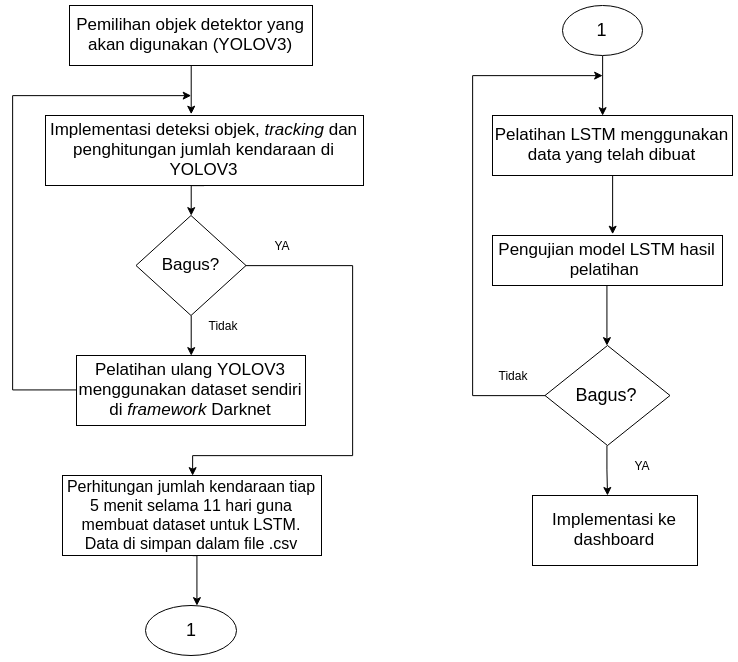
\includegraphics[scale=0.4]{Get_Model_Scheme}
	\caption{Keseluruhan proses untuk mendapatkan model terbaik}
	\label{get_model_scheme}
\end{figure}

\subsection{Deteksi, \textit{tracking}, dan \textit{counting} objek}
Pada bagian ini akan dibahas mengenai perancangan sistem dari segi Deteksi, \textit{tracking}, dan \textit{counting} objek.
\subsubsection{Deteksi Objek}
Berdasarkan gambar \ref{get_model_scheme}, proses pertama yang dilakukan adalah pemilihan jaringan objek detektor. Seperti yang telah disebutkan pada bagian dasar teori, terdapat beberapa jaringan objek detektor yang telah dikembangkan oleh ilmuan. 
Gambar \ref{yolo_comparison} menunjukan perbandingan performa dari beberapa jaringan objek detektor yang ada saat ini.
\begin{figure}
	\centering
	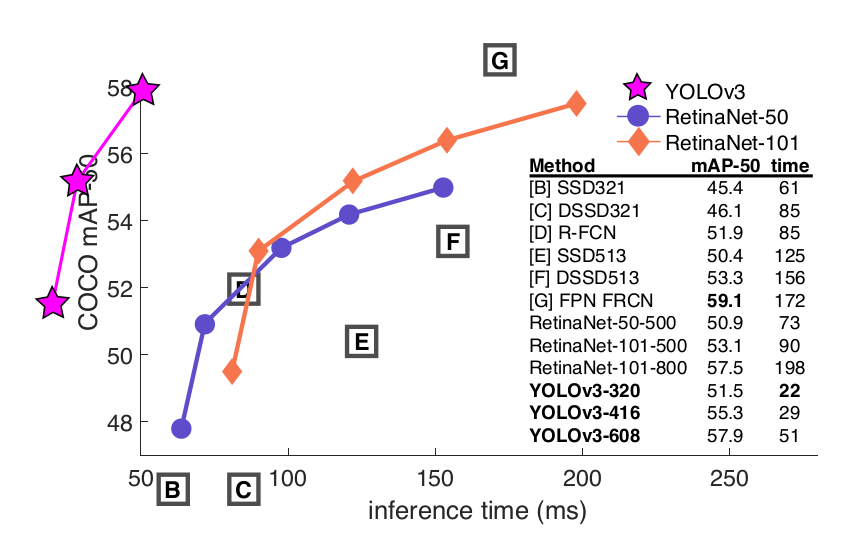
\includegraphics[scale=0.4]{YOLO_Comparison}
	\caption{Perbedaan performa beberapa network objek detektor}
	\label{yolo_comparison}
\end{figure}

Berdasarkan perbandingan tersebut, akhirnya dipilih YOLOV3-416 sebagai objek detektor pada penelitian ini. Pertimbangan ini didasari performa YOLOV3-416 yang memiliki mAP-50 cukup tinggi dengan waktu \textit{inference} yang cukup cepat. 
mAP-50 yang cukup tinggi diperlukan agar deteksi objek yang dihasilkan baik dan akurat, waktu \textit{inference} yang cukup cepat diperlukan agar deteksi yang diberikan dapat \textit{real time}. 416 menunjukan ukuran gambar input. Ukuran gambar yang tidak terlalu besar akan mempercepat proses komputasi di GPU.

Proses berikutnya yaitu menguji performa detektor yang dipilih pada permasalahan yang akan diselesaikan. Untuk penelitian ini, YOLOV3 akan dijalankan menggunakan PyTorch. Hal ini disebabkan karena terdapat beberapa pertimbangan. Pertama, PyTorch dapat mengakomodasi file berisi bobot YOLOV3 yang memiliki ekstensi .weights. Hal ini dikarenakan YOLOV3 akan dilatih ulang pada \textit{framework} Darknet menggunakan dataset baru. \textit{Framework} lain seperti Tensorflow dan Keras tidak dapat digunakan untuk mengakses file .weights. Tensorflow membutuhkan file .ckpt atau .pb sedangkan Keras membutuhkan file .h5. Jika tidak menggunakan PyTorch maka untuk proses pelatihan ulang
tidak dapat menggunakan Darknet dan harus membuat script pelatihan sendiri. Kedua, PyTorch memberikan kemudahan dalam pemrosesan tensor sehingga mudah untuk mengolah data \textit{bounding box} hasil prediksi.
Setelah YOLOV3 diuji, ditemukan bahwa meskipun YOLOV3-416 memiliki performa yang bagus dibandingkan objek detektor lainnya, objek detektor ini memberikan hasil yang kurang optimal apabila diterapkan untuk deteksi kendaraan pada lalu lintas di Indonesia secara langsung dari cctv. Hasil deteksi YOLOV3-416 original pada lalu lintas Indonesia ditunjukkan oleh gambar \ref{yoloV3_ori}

\begin{figure}[htp]
	\centering
	\includegraphics[scale=0.5]{yoloV3}
	\caption{Hasil deteksi kendaraan oleh YOLOV3-416 pada lalu lintas Indonesia}
	\label{yoloV3_ori}
\end{figure}
Berdasarkan gambar \ref{yoloV3_ori}, YOLOV3-416 mengalami kesulitan untuk mendeteksi objek sepeda motor secara benar. Hal ini dikarenakan YOLOV3 original di latih pada dataset COCO dimana objek kendaraan sepeda motor, mobil dan yang lainnya diambil hanya pada sudut tertentu seperti tampak depan dan tampak samping. Oleh karena itu YOLOV3 akan mengalami kesulitan untuk mendeteksi objek kendaraan dari sudut cctv (tampak atas). 
Dikarenakan hasil deteksi akan digunakan pada proses perhitungan jumlah kendaraan, maka dibutuhkan objek detektor yang mampu medeteksi kendaraan degan benar terutama mobil dan sepeda motor yang menjadi kendaraan utama di lalu lintas Indonesia.

Oleh karena itu seperti gambar \ref{get_model_scheme} dilakukan proses ketiga yaitu pelatihan ulang YOLOV3. Untuk melakukan pelatihan ulang maka diperlukan dataset dari kondisi permasalahan sebenarnya. Proses pengambilan dataset dilakukan dengan cara mengumpulkan gambar-gambar yang berkaitan dengan kondisi lalu lintas di Indonesia yang dilihat dari cctv. Gambar-gambar tersebut diperoleh dari layanan \textit{live streaming} ATCS di beberapa kota. 
Setelah data terkumpul, maka dilakuakan proses pelabelan (\textit{hand labeling}) untuk membuat \textit{groundtruth}. Untuk mempercepat proses pelabelan dataset maka digunakan aplikasi LabelImg [gitHub]. LabelImg merupakan tools yang \textit{open source} di GitHub.

Data anotasi dari LabelImg akan disimpan dalam file .txt. Selanjutnya akan dilakukan pelatihan ulang YOLOV3 menggunakan dataset yang ada. Pelatihan ulang YOLOV3 dilakukan menggunakan \textit{framework} official yaitu Darknet. Untuk YOLO, Darknet membutuhkan anotasi dengan format
5 komponen yaitu \\ 
\centerline{$[kelas\_Id \hspace{3mm} x\_tengah \hspace{3mm} y\_tengah \hspace{3mm} lebar \hspace{3mm} tinggi]$}\
dari \textit{bounding box} tiap objek dalam gambar. Berikutnya yang perlu dilakukan adalah mengatur parameter pelatihan seperti inisiasi \textit{learning rate}, iterasi maksimum, iterasi awal mulai penerapan \textit{adaptive learning rate}, \textit{batch size}, serta anchor box. Semua parameter training diatur dan disimpan dalam file konfigurasi .cfg dimana file ini akan 
dipanggil saat proses pelatihan. Darknet telah menyediakan fasilitas untuk menghitung metric evaluasi model antara lain \textit{True Positive (TP), False Positive (FP), False Negative (FN), precision, recall, F1-score, IoU}, dan \textit{Mean Average Precision} (mAP).

\subsubsection{\textit{Tracking} dan \textit{counting} objek}
Tracker yang digunakan pada penelitian ini adalah \textit{Simple Online and Real-time Tracking}(SORT) [pdf sort]. Pada SORT, ketika terdapat objek yang terdeteksi, \textit{bounding box} dari objek akan digunakan untuk menentukan state target. Estimasi geometri \textit{bounding box} untuk target dilakukan dengan memprediksi lokasi berikutnya pada frame saat ini. Prediksi lokasi ini berdasarkan pada komponen kecepatan yang diselesaikan oleh Kalman Filter[pdf kalman filter].
Ketika terdapat suatu objek yang masuk atau keluar dari gambar, maka tracker akan memberikan id unik kepada objek tersebut. Tracker juga akan memperhitungkan hasil deteksi yang memiliki IoU dibawah $IoU_{min}$ dan mengelompokannya kedalam untracked objek. Setiap tracker baru akan dibandingkan dengan hasil deteksi untuk mencegah terjadinya \textit{false positive} selama proses tracking.

Proses tracking terhadap suatu objek akan dihentikan apabila objek tersebut tidak terdeteksi selama $T_{lost}$ frame. Hal ini untuk menghindari semakin besarnya jumlah tracker dan kesalahan prediksi lokasi yang dikarenakan prediksi dengan jangka waktu lama tanpa ada koreksi dari detektor. Pada SORT $T_{lost}$ diset memiliki nilai 1 dengan alasan pertama, model dengan kecepatan konstan adalah prediktor yang buruk jika dibandingkan dengan kondisi sebenarnya dilapangan sehingga diperlukan nilai $T_{lost}$ yang kecil. Kedua, SORT fokus pada tracking \textit{frame-to-frame} dikarenakan proses identifikasi ulang objek berada 
di luar ruang lingkup penelitian SORT. Ketika objek terdeteksi kembali setelah $T_{lost}$ maka proses tracking akan diulang dan objek akan diberikan id baru.
\begin{algorithm}[htp]
	\begin{algorithmic}[1]
		%\State $boxes.append([x, y, w, h])$ 
		%\State $memory[indexIDs[-1]] \leftarrow boxes[-1]$
		\If {$len(boxes) > 0$}
			\State $i \leftarrow 0$
			\For { $box \in boxes$ }
				\State $(x, y) \leftarrow (int(box[0]), int(box[1]))$
				\State $(w, h) \leftarrow (int(box[2]), int(box[3]))$
				\If {$indexIDs[i] \in previous$}
					\State $previous_box \leftarrow previous[indexIDs[i]]$
					\State $(x2, y2) \leftarrow (int(previous_box[0]), int(previous_box[1]))$
					\State $(w2, h2) \leftarrow (int(previous_box[2]), int(previous_box[3]))$
					\State $p0 \leftarrow (int(x + (w-x)/2), int(y + (h-y)/2))$
					\State $p1 \leftarrow (int(x2 + (w2-x2)/2), int(y2 + (h2-y2)/2))$
					\State $buat garis (p0, p1)$
					\If {$intersect(p0, p1, line[0], line[1])$}
						\State $counter += 1$
					\EndIf
				\EndIf
				\State $i \leftarrow i+1$
			\EndFor
		\EndIf
	\end{algorithmic}
	\caption{Proses perhitungan jumlah kendaraan}
	\label{counting_ob}
\end{algorithm}

Hasil \textit{tracking} terhadap sebuah objek yang terdeteksi memberikan informasi berupa id objek dan \textit{bounding box} objek tersebut. Informasi ini akan digunakan untuk proses perhitungan jumlah kendaraan. Proses perhitungan dilakukan dengan memasangkan setiap id objek dengan \textit{Bounding box} objek tersebut. 
Id objek dan \textit{bounding box} hasil \textit{tracking} pada $T_{frame-1}$ akan disimpan. Apabila pada \textit{tracking} di $T_{frame}$ id objek yang sama memiliki \textit{bounding box} baru, maka akan dibuat suatu garis penghubung antara koordinat titik tengah \textit{bounding box} baru dengan titik tengah \textit{bounding box} lama. Garis ini
yang akan digunakan untuk menghitung objek tersebut dengan mengecek apakah garis ini bersinggungan dengan garis acuan atau tidak. Proses perhitungan ini dijabarkan pada algoritma \ref{counting_ob}.

Berdasarkan algoritma \ref{counting_ob} diketahui bahwa agar suatu objek dapat terhitung maka objek tersebut harus melewati garis acuan perhitungan dan garis pada objek harus bersinggungan dengan garis acuan tersebut. 
Untuk menentukan apakah dua buah garis bersinggungan atau tidak, dilakukan dengan menentukan formasi 3 dari 4 titik dua garis yang bersinggungan terlebih dahulu kemudian membawa konsep formasi ini untuk pengambilan keputusan. 

Formasi acuan yang digunakan adalah formasi \textit{counterclockwise} (ccw). Misalkan terdapat titik A, B, dan C seperti pada gambar \ref{ccw_img}. Tiga titik tersebut dapat dikatakan memiliki formasi ccw jika \textbf{\textit{gradien garis AC > gradien garis AB}}
sehingga harus memenuhi persamaan \ref{ccw_eq}.
\begin{equation} \label{ccw_eq}
	(C_y - A_y)*(B_x - A_x) > (B_y - A_y)*(C_x - A_x)
\end{equation}

\begin{figure}[htp]
	\centering
	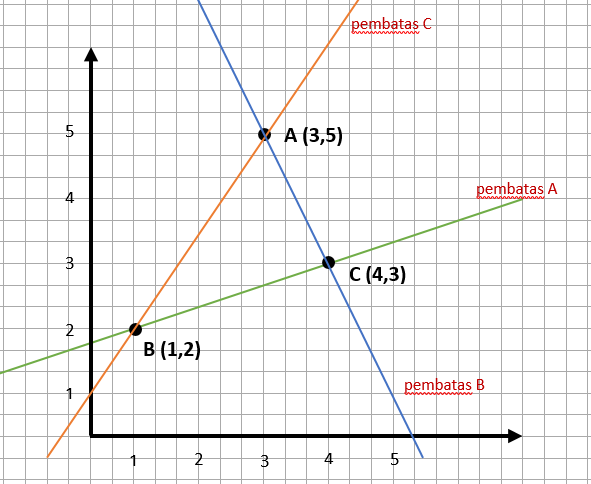
\includegraphics[scale=0.5]{CCW}
	\caption{Ilustrasi formasi 3 titik secara \textit{counterclockwise}}
	\label{ccw_img}
\end{figure}
Pada gambar \ref{ccw_img}, apabila salah satu titik tidak melewati garis pembatasnya (2 titik lain tetap berada pada posisinya), maka persamaan \ref{ccw_eq} akan selalu terpenuhi dan formasi akan selalu ccw.

Berikutnya, konsep formasi akan digunakan untuk menentukan keputusan apakah dua buah garis bersinggungan atau tidak. Berdasarkan gambar \ref{intersect_img}, maka dapat dilihat bahwa garis AB dan garis CD akan bersinggungan \textbf{\textit{jika dan hanya jika titik C dan D dipisahkan oleh garis AB}}.
Jika titik A dan B dipisahkan oleh garis CD, maka ACD dan BCD, ADC dan BDC, CAD dan CBD, DAC dan DBC memiliki orientasi yang berbeda. Begitu juga apabila titik C dan D dipisahkan oleh garis AB maka ACB dan ADB, CAB dan DAB, CBA dan DBA, BAC dan BAD memiliki orientasi yang berbeda. Dari berbagai kombinasi tersebut cukup diambil masing-masing satu saja.
Jika dirumuskan secara matematis menjadi persamaan \ref{intersect_eq}.
\begin{equation} \label{intersect_eq}
	ccw(A,C,D) =! ccw(B,C,D) \hspace{5mm} and \hspace{5mm} ccw(A,B,D) =! ccw(A,B,C)
\end{equation}
Sehingga apabila dua buah garis saling bersingungan persamaan \ref{intersect_eq} akan memberikan nilai benar.
\begin{figure}[htp]
	\centering
	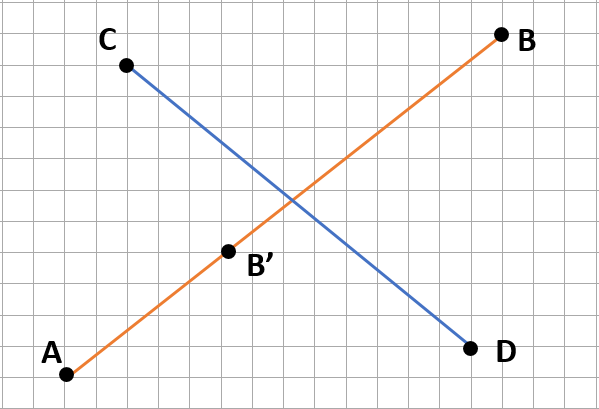
\includegraphics[scale=0.5]{intersect}
	\caption{Ilustrasi 2 buah garis yang saling bersinggungan}
	\label{intersect_img}
\end{figure}

Perhitungan jumlah kendaraan dilakukan setiap 5 menit, kemudian hasil perhitungan akan di simpan pada file .csv dengan format waktu perekaman, jumlah kendaraan per kelas, dan jumlah kendaraan total. Perhitungan dilakukan selama (satu/dua) minggu penuh guna menyediakan data latih untuk network LSTM.  

\subsection{Prediksi Arus Lalu Lintas menggunakan LSTM}
Langkah yang dilakukan untuk dapat melakukan prediksi menggunakan LSTM dibagi menjadi dua bagian, yaitu proses pelatihan (\textit{training}) dan pengujian (\textit{testing}).

\subsubsection{Proses Pelatihan (\textit{Training})}
Alur tahapan pada proses ini dijabarkan seperti pada gambar \ref{lstm_training}.
\begin{figure}
	\centering
	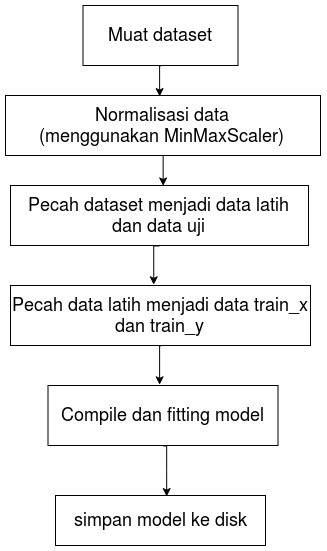
\includegraphics[scale=0.5]{Training_lstm}
	\caption{Tahapan pada proses pelatihan (\textit{training})}
	\label{lstm_training}
\end{figure}
Dataset dimuat dari file csv yang berisi data jumlah kendaraan. Data yang dipakai hanyalah data jumlah total kendaraan. Setelah itu, dilakukan normalisasi data menggunakan module MinMaxScaler dari \textit{library} scikit-learn. Normalisasi akan membuat data memiliki nilai pada rentang 0 dan 1. Hal ini dapat mempercepat proses pelatihan untuk menemukan \textit{global minima}.
Setelah di normalisasi, dataset akan dibagi menjadi data latih (\textit{train}) dan data uji (\textit{testing}). Data latih akan digunakan untuk mempelajari pola hubungan antar data dan membentuk runtun data latih input ($train\_x$) dan data latih output ($train\_y$). Proses untuk membuat data $train\_x$ dan $train\_y$ menggunakan konsep \textit{sliding window} seperti yang dijabarkan pada algoritma \ref{train_xy}. Sedangkan data uji (\textit{testing}) digunakan untuk validasi model yang telah dibuat.

\begin{algorithm}[htp]
	\begin{algorithmic}[1]
	\Function{to_supervised}{$train, n\_input, n\_out$}
		\State $data \leftarrow train.reshape(train.shape[0]*train.shape[1], train.shape[2])$
		\State $X, Y \leftarrow list(), list()$
		\State $x\_input \leftarrow 0$
		\For { $\_\in range(len(data)$ }
			\State $in\_end \leftarrow in\_start + n\_input$
			\State $out\_end \leftarrow in\_end + n\_out$
			\If {$out\_end <= len(data)$}
				\State $x\_input \leftarrow data[in\_start: in\_end, 0]$
				\State $x\_input \leftarrow x\_input.reshape((len(x\_input), 1))$
				\State $X.append(x\_input)$
				\State $Y.append(data[in\_end:out\_end, 0])$
			\EndIf
		\EndFor
	\EndFunction
	\end{algorithmic}
	\caption{Bentuk data train_x dan train_y}
	\label{train_xy}
\end{algorithm}
	
Pada proses ini, akan dilakukan pelatihan dengan memvariasikan beberapa parameter jaringan LSTM antara lain jumlah runtun data input dan output, jumlah lapisan LSTM yang digunakan serta jumlah neuron per lapisan LSTM. 
Masing-masing model ini akan masuk tahap pengujian untuk dievaluasi.

\subsubsection{Proses Pengujian (\textit{Testing})}
Alur tahapan pada proses pengujian ini dijabarkan seperti pada gambar \ref{lstm_testing}
\begin{figure}[htp]
	\centering
	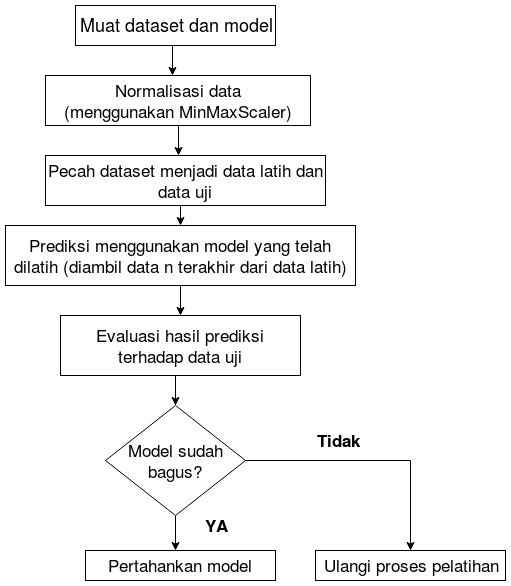
\includegraphics[scale=0.5]{Testing_lstm}
	\caption{Tahapan pada proses pengujian (\textit{testing})}
	\label{lstm_testing}
\end{figure}
Tahap pertama memuat dataset dan model yang telah dilatih pada tahap sebelumnya. Selanjutnya data dinormalisasi, kemudian dibagi menjadi data latih dan data uji sama pada proses pelatihan (\textit{training}).
Tahap berikutnya merupakan tahapan untuk mengevaluasi model yang telah dilatih. Evaluasi dilakukan dengan membandingkan hasil prediksi dengan data uji sebagai \textit{groundtruth}. Pada proses evaluasi ini, metric yang digunakan adalah \textit{Mean Average Percentage Error}(MAPE) dan \textit{Root Mean Squared Error}(RMSE). Kedua metric ini digunakan karena keluaran yang dihasilkan langsung menunjukan seberapa besar kesalahan prediksi dibandingkan data uji. 

Untuk mendapatkan hasil prediksi, dilakukan dengan mengambil sebanyak $n\_input$ data dari data latih. Data ini akan menjadi input untuk LSTM. LSTM pada Keras membutuhkan input array 3 dimensi yang memiliki bentuk ($N, W, F$) dimana $N$: jumlah runtun, $W$: panjang runtun data input, dan $F$: adalah jumlah fitur setiap runtun sehingga data input harus di\textit{reshape} menjadi bentuk seperti yang diperbolehkan.
Proses tersebut dilakukan di dalam sebuah perulangan. Tiap iterasi akan menghasilkan array hasil prediksi. Selain itu pada setiap akhir iterasi, data input akan digabung dengan data uji (sesuai indeks iterasi). Proses lebih jelas dijabarkan pada algoritma \ref{test_LSTM}.
\begin{algorithm}[htp]
	\begin{algorithmic}[1]
	\Function{get_prediction}{$train, test, n\_input$}
		\State $model \leftarrow get\_model()$
		\State $data\_input \leftarrow array(train)$
		\State $data\_input \leftarrow data\_input.reshape$
		\State $prediction \leftarrow list()$
		\For { $i \in range(len(test))$ }
			\State $data \leftarrow data\_input$
			\State $input\_x \leftarrow data[-n\_input:,0]$
			\State $input\_x \leftarrow input\_x.reshape((1, len(input\_x), 1))$
			\State $yhat \leftarrow model.predict(input\_x, verbose=0)$
			\State $yhat\_sequence \leftarrow yhat[0]$
			\State $predictions.append(yhat\_sequence)$
			\State $test\_append = test[i, :]$
			\State $data\_input \leftarrow np.append(data\_input, test\_append, axis=0)$
		\EndFor
	\EndFunction
	\end{algorithmic}
	\caption{Proses prediksi menggunakan LSTM}
	\label{test_LSTM}
\end{algorithm}

\begin{algorithm}[htp]
	\begin{algorithmic}[1]
	\Function{rekursif_prediction}{$data\_input, num\_pred, n\_input, model$}
		\State $predictions \leftarrow list()$
		\For { $i \in range(num\_pred)$ }
			\State $data \leftarrow data\_input$
			\State $input\_x \leftarrow data[-n\_input:,0]$
			\State $input\_x \leftarrow input\_x.reshape((1, len(input\_x), 1))$
			\State $yhat \leftarrow model.predict(input\_x, verbose=0)$
			\State $yhat\_sequence \leftarrow yhat[0]$
			\State $predictions.append(yhat\_sequence)$
			\State $prediction\_array \leftarrow array(predictions)$
			\State $prediction\_array \leftarrow prediction\_array.reshape((i+1)*130, 1)$
			\State $pred\_append \leftarrow prediction\_array[-130:,0]$
			\State $pred\_append \leftarrow pred\_append.reshape(pred\_append.shape[0], 1)$
			\State $data\_input \leftarrow np.append(data\_input, pred\_append, axis=0)$
		\EndFor
		\State $predictions\_result \leftarrow array(predictions)$
	\EndFunction
	\end{algorithmic}
	\caption{Proses prediksi menggunakan metode rekursif}
	\label{recursive_LSTM}
\end{algorithm}
Model LSTM yang dilatih hanya memiliki output 1, 65 dan 130 (1 hari) runtun data. Apabila ingin dilakukan prediksi untuk jangka waktu 2 hari atau bahkan 6 hari kedepan, maka menggunakan model yang sudah dilatih dapat dilakukan prediksi berdasarkan strategi rekursif.
Hasil prediksi pada timestep $t$ akan digunakan sebagai input untuk prediksi di timestep $t+1$. Proses akan terus diulangi hingga jangka waktu prediksi yang dikehendaki. Metode rekursif ini digunakan ketika implementasi langsung dilapangan.
Sebagai gambaran, untuk memprediksi 3 hari kedepan dibutuhkan data 1 hari dan 2 hari kedepan. Kenyataannya, pada implementasi riil data 1 hari dan 2 hari kedepan juga belum tersedia sehingga menggunakan hasil prediksi hari ke 1 dan ke 2 sebagai input untuk prediksi hari ke 3.
Karena menggunakan metode rekursif maka error akan semakin besar untuk jangka waktu prediksi yang panjang.
Proses pada prediksi dengan metode rekursif ini dijelaskan pada algoritma \ref{recursive_LSTM}.

Setelah model terbaik dari objek detektor dan model LSTM diperoleh, model ini akan digunakan pada proses implementasi sistem. Proses implementasi serta pengiriman dan penerimaan data dari satu proses ke proses yang lain dijabarkan pada gambar \ref{implementasi_sistem}.
\begin{figure}[htp]
	\centering
	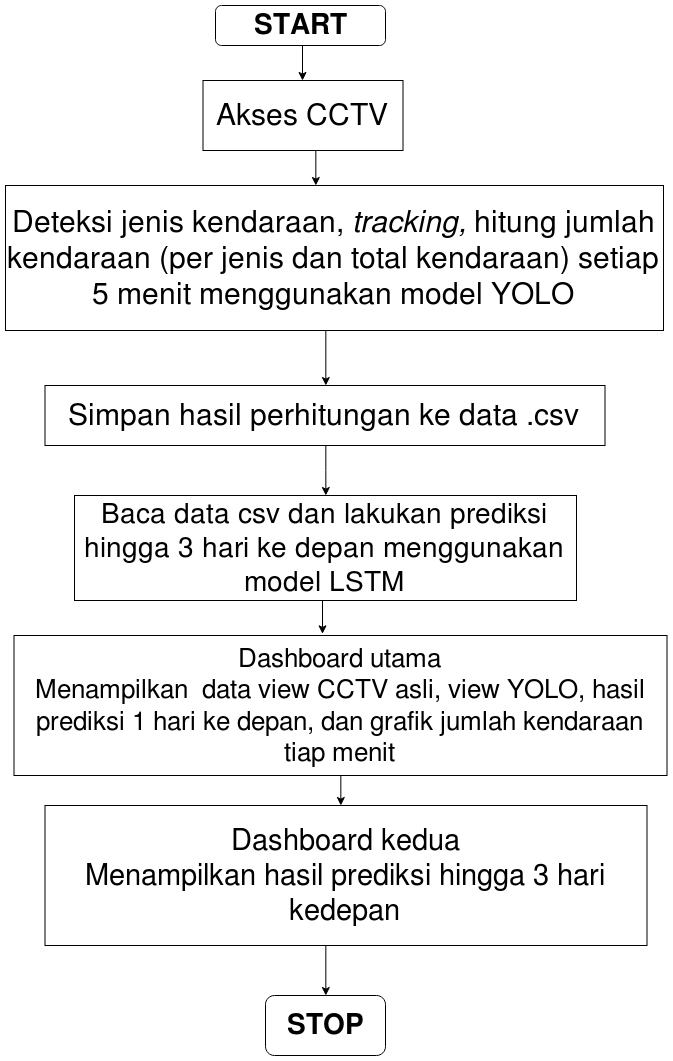
\includegraphics[scale=0.35]{Proses_Sistem}
	\caption{Urutan proses implementasi menggunakan model yang telah diperoleh}
	\label{implementasi_sistem}
\end{figure}
Data kondisi lalu lintas \textit{real-time} diakses secara \textit{live-streaming} dari CCTV yang tersedia pada layanan ATCS kota Semarang. Untuk menghindari penumpukan proses dalam satu perintah, maka dilakukan pembagian proses terutama dalam hal \textit{streaming} video.
Pembagian proses ini dapat dengan mudah dilakukan menggunakan \textit{library} ZeroMQ. 
Terdapat \textit{script} Python yang berperan khusus melakukan \textit{streaming} video kemudian mengirimkan video tersebut dalam format \textit{string} ke dua port penerima yaitu model YOLO dan \textit{dashboard} utama. Pada model YOLO, kendaraan yang berada di dalam video asli CCTV akan dideteksi, diberi \textit{bounding box}, di\textit{tracking} dan dihitung jumlah kendaraan sesuai jenisnya tiap 5 menit.
Dari YOLO, video yang telah dikenai objek detektor dikirimkan ke \textit{dashboard} utama. Selain itu YOLO juga mengirimkan hasil perhitungan jumlah kendaraan tiap 5 menit ke \textit{dashboard} utama untuk memberikan status kondisi lalu lintas. Diwaktu yang sama, jumlah kendaraan tiap 5 menit tersebut juga disimpan di dalam file csv. 
Model LSTM akan mengakses file csv ini untuk melakukan 2 prediksi yaitu prediksi 1 hari kedepan menggunakan strategi \textit{multi output} dan prediksi 3 hari kedepan menggunakan strategi rekursif \textit{multi-step}. Hasil prediksi 1 hari kedepan menggunakan strategi \textit{multi output} akan ditampilkan di \textit{dashboard}. Sedangkan hasil prediksi 3 hari kedepan menggunakan strategi rekursif \textit{multi-step}
akan ditampilkan di \textit{dashboard} kedua.


\end{document}
